\documentclass[conference]{IEEEtran}
\IEEEoverridecommandlockouts
% The preceding line is only needed to identify funding in the first footnote. If that is unneeded, please comment it out.
\usepackage{cite}
\usepackage{amsmath,amssymb,amsfonts}
\usepackage{algorithmic}
\usepackage{graphicx}
\usepackage{textcomp}
\usepackage{xcolor}
\usepackage{verbatim}
\usepackage{tabto}
\usepackage{mathtools, nccmath}
%KHOA BEGIN
\usepackage{multirow}
\usepackage{array}
%KHOA END
\usepackage[top=0.75in, bottom=1in, left=1in, right=1in]{geometry}

\ifCLASSOPTIONcompsoc
    \usepackage[caption=false, font=normalsize, labelfont=sf, textfont=sf]{subfig}
\else
\usepackage[caption=false, font=footnotesize]{subfig}

\def\BibTeX{{\rm B\kern-.05em{\sc i\kern-.025em b}\kern-.08em
    T\kern-.1667em\lower.7ex\hbox{E}\kern-.125emX}}
\begin{document}

\title{Improving Ultra-Reliable Low-Latency Communication in multiplexing with Enhanced Mobile Broadband in grant-free resources\\
%{\footnotesize \textsuperscript{*}Note: Sub-titles are not captured in Xplore and
%should not be used}
%\thanks{Identify applicable funding agency here. If none, delete this.}
}

\author{\IEEEauthorblockN{Trung-Kien Le$^{\dagger}$, Umer Salim$^{\star}$, Florian Kaltenberger$^{\dagger}$}
\IEEEauthorblockA{$^{\dagger}$EURECOM, Sophia-Antipolis, France \\
%\textit{name of organization (of Aff.)}\\
$^{\star}$TCL Mobile, Sophia-Antipolis, France \\
Trung-Kien.Le@eurecom.fr}
%\and
%\IEEEauthorblockN{Umer Salim}
%\IEEEauthorblockA{\textit{TCL Communication} \\
%\textit{name of organization (of Aff.)}\\
%Paris, France \\
%Emails: umer.salim@tcl.com}
%\and
%\IEEEauthorblockN{3\textsuperscript{rd} Given Name Surname}
%\IEEEauthorblockA{\textit{dept. name of organization (of Aff.)} \\
%\textit{name of organization (of Aff.)}\\
%City, Country \\
%email address}
%\and
%\IEEEauthorblockN{4\textsuperscript{th} Given Name Surname}
%\IEEEauthorblockA{\textit{dept. name of organization (of Aff.)} \\
%\textit{name of organization (of Aff.)}\\
%City, Country \\
%email address}
%\and
%\IEEEauthorblockN{5\textsuperscript{th} Given Name Surname}
%\IEEEauthorblockA{\textit{dept. name of organization (of Aff.)} \\
%\textit{name of organization (of Aff.)}\\
%City, Country \\
%email address}
%\and
%\IEEEauthorblockN{6\textsuperscript{th} Given Name Surname}
%\IEEEauthorblockA{\textit{dept. name of organization (of Aff.)} \\
%\textit{name of organization (of Aff.)}\\
%City, Country \\
%email address}
}

\maketitle

\begin{abstract}
In uplink (UL) transmission, the Ultra-Reliable Low-Latency Communication (URLLC) users (UEs) might be assigned the grant-free (GF)/configured-grant (CG) periodic resources to transmit data straightaway instead of sending scheduling
request (SR) and receiving UL grant. However, when these resources are not in use by the URLLC traffic, the base station (called gNB) can dynamically schedule the Enhanced Mobile Broadband (eMBB) UEs to transmit in the GF resources to increase the resource efficiency. This may lead to potential collision and detrimental QoS for URLLC as some of the URLLC UEs may become active and try to use the same resource assigned to an eMBB UE. In this paper, a two-step strategy containing an overlap indication and explicit Hybrid automatic repeat request (HARQ) feedback is proposed to improve URLLC performance in multiplexing with eMBB. Besides the explicit HARQ feedback structure, a scheme with an additional SR is also presented. Simulation results show that these two schemes help achieving URLLC requirements by reducing error probability due to Demodulation Reference Signal (DMRS) miss-detection while allowing better resource efficiency.
\end{abstract}

\begin{IEEEkeywords}
5G, URLLC, uplink scheduling scheme, eMBB and URLLC multiplexing, grant-free resources
\end{IEEEkeywords}

\section{Introduction} \label{I}
One main target of the 5G New Radio (NR) standard is to support URLLC for devices requiring low latency and high link reliability. In \cite{b6}, The 3rd Generation Partnership Project (3GPP) defines targets for the URLLC scenario: ``A general URLLC reliability requirement for one transmission of a packet is 10\textsuperscript{-5} for 32 bytes with a user plane latency of 1 ms''. The next release of 3GPP will have higher requirements of URLLC: ``Higher reliability (up to 10\textsuperscript{-6}), higher availability, short latency in the order of 0.5 to 1 ms, depending on the use cases (factory automation, transport industry and electrical power distribution)''\cite{b8}.

\subsection{Techniques accepted in 3GPP Release 15}\label{IAA}
3GPP Release 15 specified new features in physical layer design to help URLLC achieve its requirements.

Subcarrier spacings (SCS) has a flexible range from 15 kHz to 240 kHz in 5G that results in very short symbol and slot timings\cite{ad2}. In addition, the transmission is scheduled in  mini-slot level in both UL and downlink (DL)\cite{ad3}. Due to these features, the network becomes very reactive to UEs' UL and DL traffic demands and the response time to accommodate DL or UL traffic is very small compared to Long-Term Evolution (LTE) and LTE-Advanced.

Another feature is the standardization of the GF/CG UL transmissions which allows the UEs to transmit data in UL without having to transmit an explicit SR and receiving an UL grant to reduce latency \cite{ad4}.

\subsection{Problem of multiplexing URLLC and eMBB in GF resources}\label{IBB}
In 5G, as mentioned in Section \ref{IAA}, the gNB can schedule GF resources for URLLC UEs but it does not have any prior information which of these GF resources will actually be used by URLLC UEs or which of the UEs in the group configured to the resources will use a specific resource. If the cell is loaded and the gNB schedules some eMBB UEs on the resource overlapping with CG occasion, as shown in Fig.~\ref{fig1}, there is going to be transmission collision of dynamically scheduled eMBB and URLLC GF transmissions. 

\begin{figure}[htbp]
\centerline{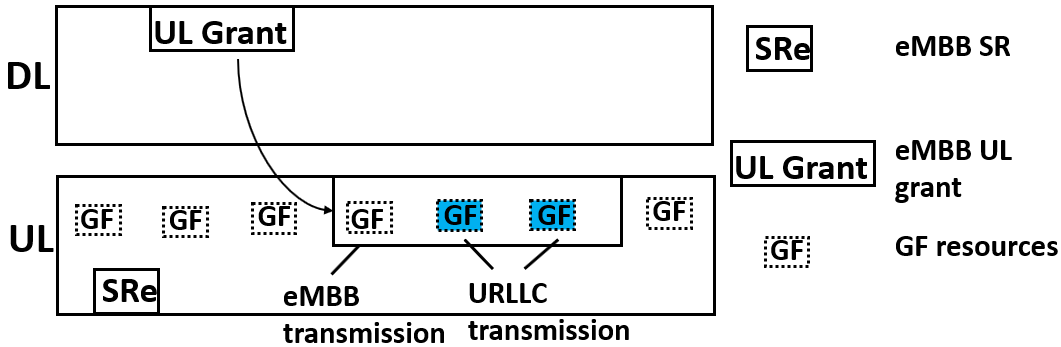
\includegraphics[scale=0.25]{fig1.PNG}}
\caption{A collision of UL URLLC GF transmission with eMBB transmission in case of Frequency Division Duplex (FDD).}
\label{fig1}
\vspace{-3mm}
\end{figure}

When the transmissions from eMBB and URLLC UEs in GF resources overlap, it results in lower decoding probability due to lower resulting SINR for both UEs. This can be a serious problem for URLLC UEs in particular due to their tight latency and reliability targets.

In case the gNB is able to identify the URLLC UE from its DMRS sequence, it may try to quickly reschedule the UE over non-overlapping resources if an error happens.

The increased interference due to overlapping transmissions of eMBB and URLLC UEs may lead to a catastrophic situation when the gNB may not even identify the URLLC UE (DMRS miss-detection). The current HARQ structure in UL transmission for NR is timer based, which means that upon transmission of packet, the UE will start the HARQ timer. If it receives an UL grant for the re-transmission of the same transport block (TB) from the gNB, it does the retransmission over the resources scheduled in the UL grant. If it receives no UL grant from the gNB and the HARQ timer expires, it considers that the TB was successfully decoded at the gNB and discards the data in the buffer. 

The timer-based HARQ feedback and UL GB retransmission are standardized because this minimizes the control overhead for sending HARQ feedback. This is reasonable in general but in the cases of dynamic UL multiplexing, giving rise to overlapping transmissions with GF UEs, when the gNB will not be able to identify the UEs transmitting on GF resources, the UEs will discard their packets and consider the successful detection that leads to serious performance degradation for URLLC UEs.

\subsection{Prior art}\label{ICC}
In \cite{b2} and \cite{b3}, when there is an overlap, the gNB asks the URLLC UE to apply a different pre-configured transmission power that is higher than power level used in case of no overlap. However, an increase of power causes an interference among the neighboring cells. Secondly the cell-edge UEs may be power limited and cannot raise their transmission power. This is also the problems of \cite{b5} when the gNB assigns URLLC physical uplink shared channel (PUSCH) with updated transmission parameters such as resource, MCS, transmit power, etc. on GF resources that are occupied by eMBB PUSCH. 

In \cite{b7}, the group common control channel reveals resource range allocated to GB eMBB UE so the GF UE can exclude the occupied resource. Nevertheless, the GF UE has less resources left to transmit than the original configured resources so this partial transmission may not be decodable at the gNB.

In \cite{b9}, the gNB informs the URLLC UE which of the GF resource set has overlapping eMBB transmission such that the URLLC UE can initiate the GF transmission over resources not occupied by the ongoing eMBB transmission. It might result in high latency if all resources in the current occasion are full and the UE must wait until the next transmission occasion.

A preemptive scheme in \cite{b10} cannot be applied in URLLC GF transmission because the gNB does not know the URLLC transmission in advance to preempt eMBB transmission.

A successive interference cancellation (SIC) receiver in \cite{b11} only benefits eMBB UE rather than URLLC UE because URLLC data is decoded first due to latency requirement.

In this work, a multiplexing scheme with two-step strategy is presented in Section \ref{II}. The first step comprises of the gNB transmitting an overlap indication whenever it schedules an UL transmission having an overlap with the resources configured to the GF transmissions. The second step of the proposed strategy comprises of making the overlapped transmissions to use explicit HARQ feedback structure. An alternative way of the second step is to make the gNB indicate the UEs to send SR in parallel to data transmitted on the GF resources to improve the reliability. Section \ref{III} shows numerical results and performance evaluation. Finally, Section \ref{IV} is conclusion.

\section{Strategy to multiplex the eMBB and URLLC UEs}\label{II}

\subsection{Overlap indication and explicit HARQ acknowledgement (ACK) feedback}\label{IIAA}

This paper proposes two-step strategy to overcome the problem of the multiplexed UL eMBB and URLLC transmissions. In the first step, upon scheduling a GB transmission of the eMBB UE over the GF resources, the gNB sends an indication of resource overlap to the URLLC UEs. As the gNB does not know which of the URLLC UEs configured for GF resources may become active in the current interval, this indication needs to be sent to all UEs who have been configured with the GF resources in the overlapping interval as illustrated in Fig.~\ref{fig2}. Upon receiving this overlap indication, the URLLC UEs are aware of the resources which have been dynamically scheduled for other UEs and in case of transmission,  their transmissions will be received with an increased interference.

\begin{figure}[htbp]
\centerline{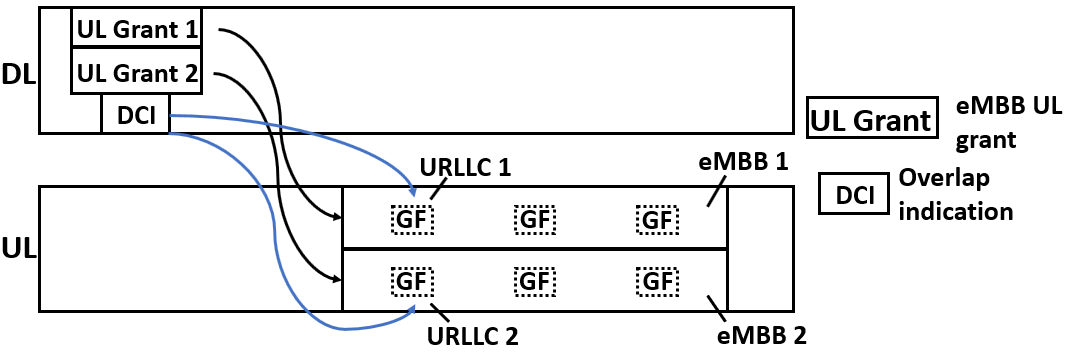
\includegraphics[scale=0.22]{fig2.PNG}}
\caption{Signalling the URLLC UEs about an overlap with the eMBB UEs in GF regions.}
\label{fig2}
\vspace{-2mm}
\end{figure}

The second step of the proposed strategy comprises of making the overlapping transmissions use explicit HARQ feedback structure rather than legacy timer-based feedback. The resource overlap indication can serve this purpose by containing a 1-bit flag to tell if the feedback becomes explicit or not. Upon receiving this indication, the URLLC UEs, who transmit on the overlapping resources, expect to receive explicit HARQ feedback from the gNB for their transmissions. 

Thereby, within a configured time period, the GF UEs receive either explicit HARQ ACK indicating the successful detection of their TB or UL grant for re-transmission in case the gNB failed to decode the TB but was able to identify the transmitting UE.  For the third case, if the gNB even fails to identify the UE due to high interference (DMRS miss-detection), it cannot schedule the UE for a re-transmission in the conventional timer-based feedback so the UE assumes that a packet is decoded correctly and drops it from buffer to transmit the next packet. This is the scenario where our proposed explicit HARQ feedback becomes the most promising. If the GF UE receives neither an ACK nor an UL grant within a configured time, the UE does not consider that its data is successful, rather it considers that the gNB failed to identify its identity (ID) due to high interference in the overlapping transmissions and retransmits the TB on the subsequent GF resources. Table~\ref{tab3} summarizes the operation of conventional timer-based feedback structure and explicit feedback structure.

\begin{table}[htbp]
\caption{Comparison of different feedback structures}
\begin{center}
\begin{tabular}{|p{8em}|p{7em}|p{7em}|}
 \hline
 \textbf{Case} & \textbf{Timer-based feedback}&\textbf{Explicit feedback}\\
 \hline
 DMRS: detected&No ACK/UL grant&ACK\\TB: decoded & &\\
 \hline
  DMRS: detected&UL grant: &UL grant:\\TB: failed & reschedule&reschedule\\
 \hline
DMRS: failed&No ACK/UL grant: packet lost&No ACK/UL grant: packet retransmitted automatically\\

%  increase row height, number of & = number of collumn
% &&&&&\\[-1em]
 
 \hline
\end{tabular}
\label{tab3}
\end{center}
\vspace{-4mm}
\end{table}

%In addition, the URLLC transmission can be made to stop immediately after receiving an explicit HARQ feedback. Thus, the URLLC UE does not need to carry out all repetitions as configured in parameter repK from higher layer. It helps the URLLC UE save power and resources. Besides, the eMBB UE also avoids suffering from an interference from the URLLC UE’s repetitions and there is more chance that the gNB is still able to decode correctly eMBB data despite the collision with URLLC data at the beginning. 

Block error rate (BLER) of a packet in timer-based feedback structure and explicit feedback structure is shown in \eqref{eq1} and \eqref{eq2} in Section \ref{III}.

The timer value, for which the UE should wait to receive ACK or UL grant, can be configured by radio resource control (RRC) parameters. This value can be selected as a function of reliability and latency targets of the UEs. For some UEs with extremely high latency and reliability targets, this timer value can be put to zero which means to do the automatic transmission in case of overlapping transmissions to maximize the chance of correct data detection at the gNB.

\begin{comment}
In one strategy, it could be decided that all the overlapping GF transmissions use explicit HARQ feedback. In this case, no explicit signalling or flag is needed to indicate the activation of explicit HARQ feedback. Thus, the GF UEs upon knowing that they will transmit on the overlapping resources expect explicit HARQ feedback. There could, though, exist some cases where the gNB knows that it has configured large number of repetitions for GF UEs or it has scheduled the dynamic UL transmission from eMBB UE with a lower power, which will result in a good probability of successful detection or at least UE identification and it decides not to change the HARQ to explicit feedback. To keep the flexible control at the network side, the overlap indication can comprise an indication, a flag, which tells if the feedback becomes explicit or not in the indicated overlapping GF occasions.
\end{comment}

\subsection{Overlap indication and additional SR}\label{IIBB}
In a variation of the proposed scheme in Section \ref{IIAA}, the second step of making the transmissions explicit HARQ feedback-based can be replaced to use an additional SR. The gNB can indicate the URLLC GF UEs by overlap indication in the first step described in Section \ref{IIAA} to send a SR in parallel for the TB transmitted over the overlapping GF resources. The SR sent to the gNB will provide a further means besides DMRS detection to detect the ID of the UE transmitting in the interfered GF transmission. When the gNB is unable to identify the UE making the GF transmission because of DMRS miss-detection, the gNB still can identify that UE by decoding the additional SR and react fast to the received SR by sending an UL grant to this UE. Thanks to the UL grant, the UE is likely to retransmit the packet and has a successful transmission in latency budget instead of assuming a successful transmission and dropping the packet as in the conventional scheme. When the gNB is able to decode the data successfully, it still reacts to SR to send some indications to the UE about the successful detection.  

Physical uplink control channel (PUCCH) and PUSCH are not allowed to be transmitted simultaneously. In case the UE needs to transmit uplink control information (UCI) while transmitting UL data on PUSCH, it sends the UCI on PUSCH. When the UE is not transmitting PUSCH, it sends the UCI carrying SR, feedback for DL data  etc, on the PUCCH resources using appropriate PUCCH format as a function of UCI content and the PUCCH configurations. The simplest strategy to send SR (which is UCI) when the URLLC UE is transmitting over overlapping GF resources would be to transmit it over PUSCH GF resources along with the transmission of the TB. This can be simple from implementation perspective but from the performance point of view, it does not help to improve significantly the performance of the UE ID detection. If DMRS of PUSCH is not detected by the gNB because of bad channel and interference from eMBB transmission, there is high chance that the gNB also cannot decode the SR to obtain the UE ID multiplexed with PUSCH. For this reason, to achieve a better UE ID detection, the SR is proposed to be transmitted using PUCCH configuration on the specified PUCCH resources separated from PUSCH. As PUCCH resources are dedicated resources on different frequency physical resource blocks (PRBs) and OFDM symbols, this provides additional diversity advantage to the SR transmitted in these resources compared to multiplexing and transmitting it over UL GF resources along with the TB. Therefore, the UE is configured to transmit this SR on PUCCH resources in parallel to the transmission of TB on the overlapping resources.

The overlap indication may have an explicit indication, in the form of a single bit flag, which may require the UEs transmitting over overlapping GF occasions to send SR. In fact, more flexibility and better performance can be achieved by having the flexible control of the explicit HARQ feedback structure and the transmission of SR. The gNB can then choose which strategy to choose in different situations. As an example, if the periodicity of current GF occasions is not very fast, it may make sense to indicate the overlapping GF UEs to send an SR. And in the cases, if the resources configured for SR are not sufficient or not in close proximity compared to the subsequent GF occasions, it may be suitable to prioritize the explicit HARQ feedback and automatic retransmission in case the UEs receive no ACK/UL grant indication for the transmitted TB.

\begin{comment}
The overlap indication can further be enhanced to modify or update some of the transmission parameters of the GF transmissions which happen to be in the overlap situations such as transmission power level or the number of repetitions. 
\end{comment}

\subsection{Configuration and Signalling for the Overlap Indication}\label{IICC}
One very important feature of the proposed scheme is that the overlap indication is sent to the UEs who have been pre-configured for the GF resources. As GF resources may be shared by multiple UEs, and the gNB has no idea a priori which of these UEs may transmit their data over GF resources, this overlap indication is sent in a group-common manner. Thus, the proposal is to send the overlap indication in a group-common downlink control information (DCI).

For UL overlap indication sent in group-common DCI, a DCI format similar to the DCI format 2\_1 in \cite{ad6} can be used. DCI 2\_1 is also used for DL pre-emption indication. The size of DCI format 2\_1 is configurable by higher layers up to 126 bits and each indication has 14 bits. 

The UL overlap indication sent to the URLLC UEs comprises of the indication of UL GF resources typically scheduled for the eMBB UEs. The eMBB UEs would be normally scheduled for the slot duration or most part of the valid UL symbols so it would be judicious to have more bits of UL reference resource field defining the frequency granularity. To keep a format close to the DL pre-emption indication and adapted to indicate the UL overlap resource, there are two possibilities of UL overlap indication. In the first design, all 14 bits are used to indicate the frequency PRB region for the whole slot. Thus, each bit in the 14-bit long bitmap indicates 1/14 of the frequency PRBs of the carrier as shown in left part of Fig.~\ref{fig3}. The second option is to split the time-frequency grid of the slot in 7 frequency zones each spanning one half slot. Thus, each bit may indicate an overlap over 1/7 of the frequency PRBs for a half slot time duration as illustrated in right part of Fig.~\ref{fig3}. 

\begin{figure}[htbp]
\centerline{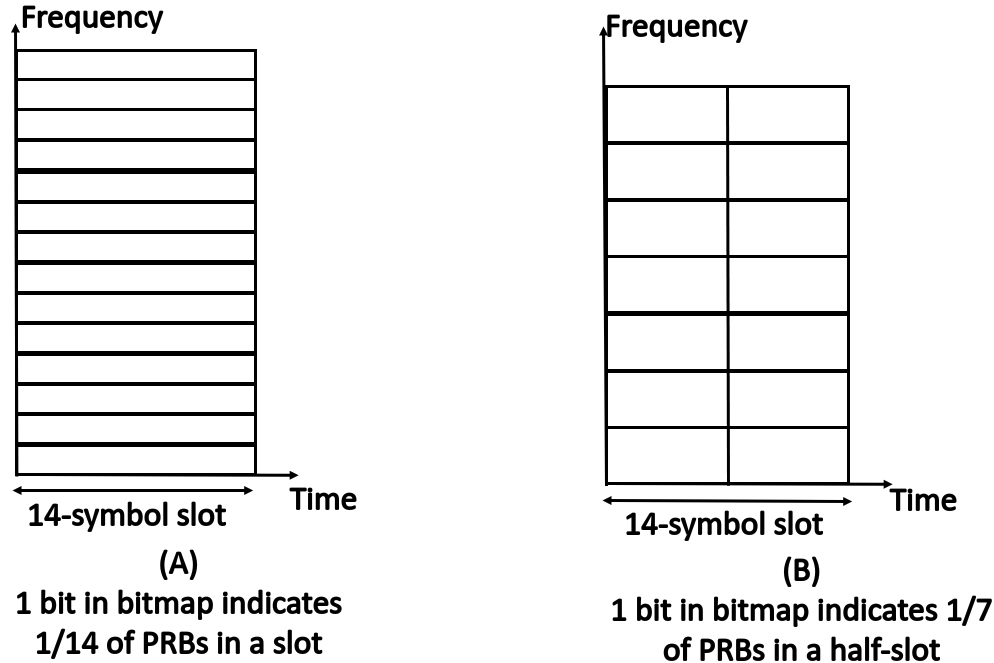
\includegraphics[scale=0.18]{fig3.png}}
\caption{Resource Indication in Uplink Overlap Indication.}
\label{fig3}
\vspace{-2mm}
\end{figure}

The UEs configured with GF resources can be configured to listen and decode the overlap indication as part of GF configuration. The activation or de-activation of this operation can be done in different ways for Type 1 and Type 2 GF as specified in \cite{ad4}. For RRC configured Type 1, the activation and de-activation can be done by RRC signalling. For configured grant Type 2, where some parameters of GF can be updated by DCI, the activation or de-activation of overlap indication can be made through DCI signalling which is used to update other GF parameters.

The overlap indication can be sent at the same time when the gNB sends the dynamic UL grant scheduling a UE over the GF resources as shown in the left part of Fig.~\ref{fig4}.

When the gNB sends an UL grant scheduling an eMBB UE, the scheduled resources are not necessarily in the same slot where UL grant is sent. Rather typically the UL grant will be for the resources located in one of the subsequent slots. If the gNB transmits the overlap indication along with the UL grant, it needs to indicate the slot where this overlap will occur. To avoid this additional signalling and to keep the treatment of UL grant simple, the overlap indication can be transmitted in the slot where overlap occurs as shown in the right part of Fig.~\ref{fig4}. However, it may not be preferable to send and receive at the same time, so transmitting the overlap indication in the DL direction in the same slot as of the overlapping CG occasions may not be very interesting. In some other cases like time division duplex (TDD) operation mode, it may be completely impossible. Thus, based on the system design, one of these two transmission schemes
is determined.

\begin{figure}[htbp]
\centerline{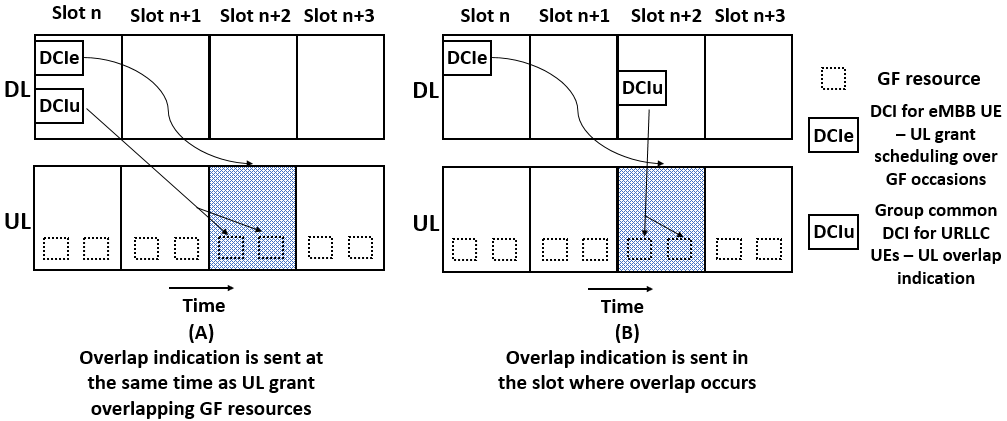
\includegraphics[scale=0.24]{fig4.PNG}}
\caption{Timing to send the UL Overlap Indication.}
\label{fig4}
\vspace{-3mm}
\end{figure}

One big advantage of sending the overlap indication to URLLC UEs is that the overlap indication is primarily indicating the overlap caused by dynamic scheduling of eMBB UEs over the CG resources. As eMBB UEs may be scheduled only once during a slot, the indication periodicity can be kept to be once per slot and no mini-slot monitoring is needed to receive the overlap indication. This is advantageous in the sense that it does not overload the UEs with additional DCI monitoring and decoding burden. 

\subsection{Design of Explicit HARQ Feedback}\label{IIDD}
In the proposed strategy, the gNB shifts the GF transmissions in the overlap region from timer-based approach to explicit-HARQ-feedback approach. Thus, a design for the explicit HARQ feedback in general may be needed. The proposal is to use DCI as an explicit HARQ feedback sent with UE specific configured scheduling-radio network temporary identifier (CS-RNTI) which is used with configured grant-based transmissions. If the gNB is able to successfully decode the data despite the overlap, it can send an UL grant to this UE with the same HARQ process number (HARQ ID) as of the successfully received TB, and the UE upon receiving this UL grant would know that this is in fact not a retransmission request but an explicit ACK for the previously transmitted TB. To avoid any confusion, new-data-indicator (NDI) field can be set to zero. Further, some of the fields in the DCI which are actually not needed, such as the time and frequency resource assignment fields, may be sent with fixed known values which can be pre-decided to be used in the ACK indication.

\section{Numerical results and performance evaluation}\label{III}


\begin{table}[htbp]
\caption{Simulation parameters}
\begin{center}
\begin{tabular}{|p{8em}|p{8em}|}
 \hline
 \textbf{Parameters} & \textbf{Values}\\
 \hline
 Waveform & CP-OFDM\\
 \hline
 Subcarrier spacing & 60kHz\\
 \hline
 Channel model & Rician\\
 \hline
 K factor & 1\\
 \hline
 Number of allocated PRB & 8\\
 \hline
 DMRS detection mechanism & Time-domain correlation\\
 

%  increase row height, number of & = number of collumn
% &&&&&\\[-1em]
 
 \hline
\end{tabular}
\label{tab1}
\end{center}
\vspace{-4mm}
\end{table}

\begin{table*}[htbp]
\caption{Performance comparison between different scenarios and schemes at SNR=$-1.4dB$, FAR=0.001, $P^{e}_{d2}$=$P^{e}_{SR}$=0.01}
\begin{center}
\begin{tabular}{|p{19em}|p{9em}|p{10em}|p{12em}|}
 \hline
 \textbf{Case} & \textbf{URLLC UE ID miss detection probability}& \textbf{Retransmission in UE ID miss detection}& \textbf{URLLC UL transmission's BLER due to the first UE ID miss detection}\\
 \hline
 No collision  & 10\textsuperscript{-5}&No&10\textsuperscript{-5}\\
 \hline
 Collision in the conventional scheme& 3.4$\times$10\textsuperscript{-4}&No&3.4$\times$10\textsuperscript{-4}\\
 \hline
 Collision with power control (\cite{b2} and \cite{b3})&2.44$\times$10\textsuperscript{-4}&No&2.44$\times$10\textsuperscript{-4}\\
 \hline
 Collision with explicit feedback (proposed)& 3.4$\times$10\textsuperscript{-4}&Yes&3.4$\times$10\textsuperscript{-6}\\
\hline
 Collision with additional SR (proposed)& 3.4$\times$10\textsuperscript{-6}&No&3.4$\times$10\textsuperscript{-6}\\

%BLER_trans=P_DMRS+(1-P_DMRS)*P_data
%  increase row height, number of & = number of collumn
% &&&&&\\[-1em]
 
 \hline
\end{tabular}
\label{tab2}
\end{center}
\vspace{-6mm}
\end{table*}

\begin{figure}[htbp]
\centerline{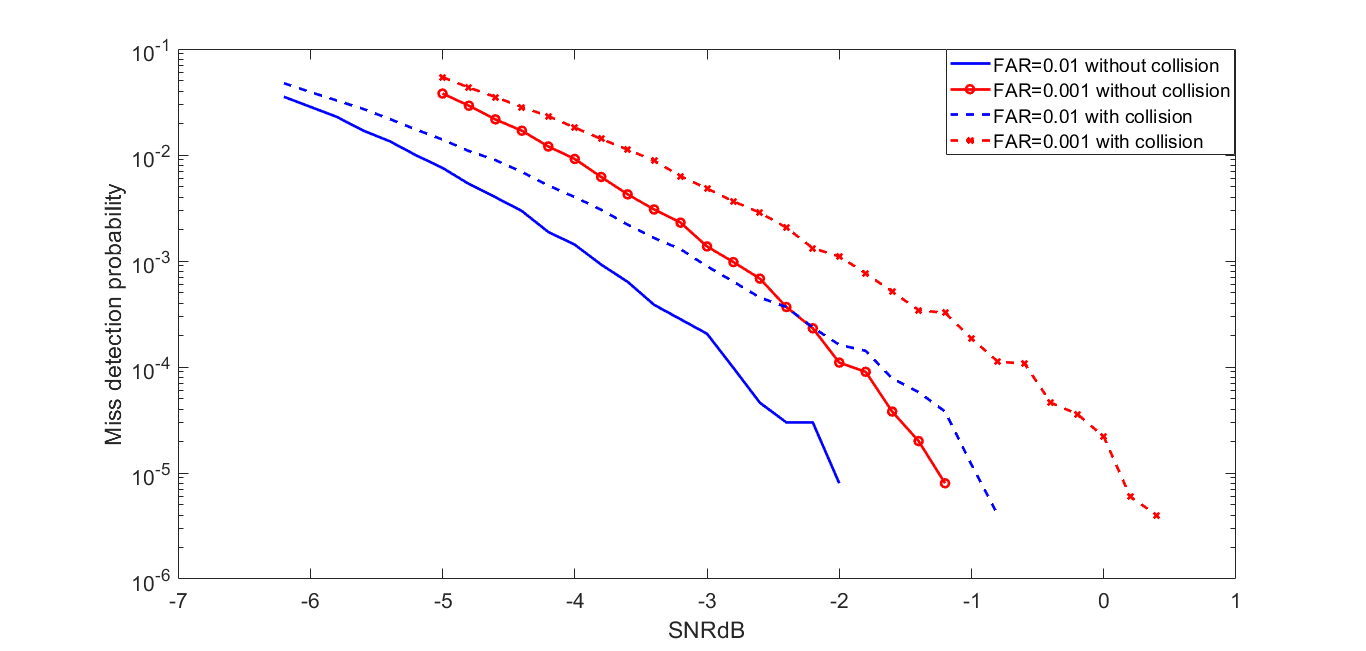
\includegraphics[scale=0.33]{fig5.png}}
\caption{DMRS detection performance.}
\label{fig5}
\vspace{-3mm}
\end{figure}

Simulation parameters are shown in Table~\ref{tab1}. Fig.~\ref{fig5} illustrates the performance of DMRS detection in three cases: the URLLC UE transmits in the GF resources without any collision with another eMBB UE, the URLLC UE has a collision with an eMBB UE at the same power level and the URLLC UE has a collision when increasing power 1dB higher than an eMBB UE. For each DMRS detection, the correlation result is compared with a threshold to determine whether DMRS exists or not. This threshold is chosen according to a target false alarm rate (FAR) indicating the cases that the gNB determines the existence of DMRS while in reality there is no DMRS transmitted. A higher threshold is required for a lower FAR but also results in more missed detection.

Due to a collision between DMRS of the URLLC UE of interest and data/DMRS of another eMBB UE, the performance of DMRS detection of the URLLC UE degrades significantly as can be seen in Fig.~\ref{fig5} and cannot achieve the miss detection probability 10\textsuperscript{-5} at the same SNR level of the case without collision. At FAR of 0.001 and SNR of -1.4dB, the miss detection probability increases from 10\textsuperscript{-5} of the case without collision to 3.4$\times$10\textsuperscript{-4} of the case with a collision with an eMBB UE at the same power. Fig.~\ref{fig5} also shows that even with power control scheme in \cite{b2} and \cite{b3} when the URLLC UE's power increases 1dB higher than the eMBB UE's power, miss detection probability is still 2.44$\times$10\textsuperscript{-4} that is higher than 10\textsuperscript{-5} of the case without collision. As DMRS detection is mandatory for channel estimation to decode data as well as for recognizing UE ID to reschedule a retransmission if necessary in conventional scheme, a degradation of DMRS detection makes the system unable to support reliability URLLC requirement. BLER of an UL transmission with one potential retransmission in the conventional scheme or power control scheme ($ P^{e}_{1}$) is calculated as\useshortskip

\begin{equation}
\begin{split}
 &P^{e}_{1} = P^{e}_{DMRS1} + \\
        &+ (1-P^{e}_{DMRS1})P^{e}_{d1}(P^{e}_{DMRS2} + (1-P^{e}_{DMRS2})P^{e}_{d2}),\label{eq1}   
\end{split}
\end{equation}
where $ P^{e}_{DMRS1}, P^{e}_{DMRS2}$ are the miss detection probabilities of the initial (with collision) and retransmitted (without collision) DMRS (see Figure \ref{fig5}), and $P^{e}_{d1}, P^{e}_{d2}$ are the error probabilities of the initial (with collision) and retransmitted (without collision) PUSCH.

In \eqref{eq1}, the first term is the error probability when the gNB cannot detect DMRS to decode or reschedule data so the UE does not retransmit data and data is lost. The second term is the error probability when the gNB detects DMRS and identifies UE ID but fails to decode data so it reschedules data. However, it cannot decode the retransmission and an error still occurs.

The usage of an explicit HARQ feedback as explained in Section \ref{IIAA} solves the problem of DMRS miss-detection in the overlapping region because it allows the UE to carry out the retransmissions in the interference-free regions even if DMRS is not detected by the gNB. BLER of an UL transmission with one potential retransmission in the proposed scheme with explicit feedback ($ P^{e}_{2}$) is calculated as\useshortskip

\begin{equation}
\begin{split}
 &P^{e}_{2} = P^{e}_{DMRS1}(P^{e}_{DMRS2} + (1-P^{e}_{DMRS2})P^{e}_{d2}) + \\
        &+ (1-P^{e}_{DMRS1})P^{e}_{d1}(P^{e}_{DMRS2} + (1-P^{e}_{DMRS2})P^{e}_{d2}).\label{eq2}   
\end{split}
\end{equation}

Compared to \eqref{eq1}, the first term in \eqref{eq2} is enhanced because of a retransmssion while the second terms are the same.

The final column in Table~\ref{tab2} shows a remarkable enhancement of the first term of error probability in UL transmission with explicit HARQ feedback in case of URLLC and eMBB multiplexing in comparison to the conventional scheme with timer-based feedback and power control scheme in \cite{b2} and \cite{b3}. Moreover, the proposed scheme can be applied to all UEs in a cell while the power control scheme to increase URLLC UEs' power cannot be applied to the cell-edge UEs because of power limitation. 

Table~\ref{tab2} also shows an improvement of UE ID detection (the first term in \eqref{eq3}) when an additional SR is transmitted in the separate PUCCH in parallel with data (PUSCH) in GF resources. As can be seen in \eqref{eq3}, the SR provides another chance for the gNB to detect UE ID. Therefore, the error probability because of DMRS miss-detection decreases. BLER of an UL transmission with one potential retransmission in the proposed scheme with an additional SR ($ P^{e}_{3}$) is calculated as\useshortskip

\begin{equation}
\begin{split}
 P^{e}_{3} &= P^{e}_{DMRS1}\times P^{e}_{SR} + \\
        &+ (1-P^{e}_{DMRS1}\times P^{e}_{SR})P^{e}_{d1}\times\\
        &\times(P^{e}_{DMRS2} + (1-P^{e}_{DMRS2})P^{e}_{d2}),\label{eq3}   
\end{split}
\end{equation}
where $P^{e}_{SR}$: the error probability of SR

The selection between two proposed schemes is explained in Section \ref{IIBB}.
 
The presence of retransmission in explicit feedback leads to latency and resource consumption but guarantees target reliability in case of DMRS miss-detection, while the conventional scheme stops the transmission straightaway and causes packet loss so latency and resource consumption have no meaning when a packet is already failed to be decoded correctly. Moreover, with SCS 60kHz and the decoding time of one transmission being 0.1ms for a packet spreading in 4 OFDM symbols, even with one retransmission, the system consumes 0.5ms in total and still satisfies the latency requirement of 1ms.

Compared to conventional scheme, overhead of explicit feedback structure is higher due to ACK signal but is limited because the explicit feedback structure is only used when there is an overlap in GF resources (a cause of high interference) and an overlap indication triggers this structure. In addition, as can be seen in Table~\ref{tab2}, the error probability in the overlapping transmissions increases so the number of ACK feedback decrease while the number of the cases without any feedback because of DMRS miss-detection increase. For this reason, a mechanism to trigger a retransmission as the proposed explicit feedback structure becomes imperative. It is the same reason that the overhead of SR transmitted in parallel with PUSCH is acceptable in eMBB and URLLC multiplexing.

\section{Conclusion}\label{IV}

This paper presents a strategy to multiplex the GB eMBB and GF URLLC transmission while guaranteeing the strict requirements of URLLC. An overlap indication is used and combined with an explicit HARQ feedback or an additional SR to help reduce the error probability of URLLC UE in case of DMRS miss-detection. The proposed scheme provides a mechanism to meet very stringent URLLC constraints with minimal additional control overhead.

\begin{thebibliography}{00}
\bibitem{b6} 3GPP TR 38.913 v15.0.0, ``Study on scenarios and requirements for next generation access technologies.''
\bibitem{b8} Huawei, HiSilicon, Nokia, Nokia Shanghai Bell, ``New SID on Physical Layer Enhancements for NR URLLC''. 3GPP RP-182089, TSG-RAN\#81, Gold Coast, Australia, Sept 10--13, 2018.
\bibitem{ad2} 3GPP TS 38.211 v15.3.0, ``Physical channels and modulation.''
\bibitem{ad3} 3GPP TR 38.802 v14.2.0, ``Study on new radio access technology physical layer aspects.''
\bibitem{ad4} 3GPP TS 38.214 v15.3.0, ``Physical layer procedures for data.''
%\bibitem{b1}  ZTE, ``On UL inter UE Tx prioritization/multiplexing'', 3GPP R1-1812389, RAN1\#95, Spokane, USA, November 12--16, 2018.
\bibitem{b2} Huawei, HiSilicon, ``UL inter-UE transmission prioritization and multiplexing'', 3GPP R1-1810158, RAN1\#94bis, Spokane, Chengdu, China, 8--12 October, 2018.
\bibitem{b3} ZTE, ``UL inter-UE multiplexing between eMBB and URLLC'', 3GPP R1-1900074, RAN1 AH 1901, Taipei,  21--25 January, 2019.
%\bibitem{b4} Sony, ``On Enhancement of UL grant-free transmissions'', 3GPP R1-1808345, RAN1\#94, Gothenburg, Sweden, August 20--24, 2018.
\bibitem{b5}  Sony, ``Inter-UE uplink multiplexing of URLLC \& eMBB traffics'', 3GPP R1-1812745, RAN1\#95, Spokane, USA, November 12--16, 2018.
\bibitem{b7}  Institute for Information Industry (III), ``UL Inter UE Tx prioritization/multiplexing'', 3GPP R1-1813481, RAN1\#95, Spokane, USA, November 12--16, 2018.
\bibitem{b9}  NEC, ``UL inter-UE multiplexing of eMBB and URLLC'', 3GPP R1-1812419, RAN1\#95, Spokane, USA, November 12--16, 2018.
\bibitem{b10}  C.-P. Li, J. Jiang, W. Chen, T. Ji, and J. Smee, ``5G ultra-reliable and low-latency systems design,'' in 2017 European Conference on Networks and Communications (EuCNC), Jun. 2017, pp. 1-5. 
\bibitem{b11} D. Tse and P. Viswanath, Fundamentals of Wireless Communication. Cambridge University Press, 2005. 
\bibitem{ad6} 3GPP TS 38.212 v15.3.0, ``Multiplexing and channel coding.''

\end{thebibliography}
\vspace{12pt}


\end{document}
